\section{Evaluation}
This section elaborates experimental results that support the models and formulations shown in section 3. In section 5.1, we describe the evaluation setting including hardware and software architecture, and prototype pipe system. Section 5.2 describes measured vibration on a pipe and its mapping to the actual water flow rate in the pipe. It evaluates its performance against the ground truth obtained from the water flow meter. Section 5.3 shows the end result of the system. 

\subsection{ Deployment Setting System Architecture}
As shown in Figure ??, the design of the NAWMS system consists of tiered sensor system and a custom pipe system. The pipe system is made of one main pipe and three branches; one branch is ?? copper pipe, one is ?? size PVC pipe and the other one is ?? size PVC pipe. The main pipe is equipped with an commercial water flow meter that generates pulse train whose pulse speed is proportional to the actual flow rate. Each branch is equipped with an acceleration sensor that is a part of MTS310 sensor board. MicaZ is used to collect and process sensor data and is running SOS operating system[]. The vibration mote samples acceleration perpendicular to the pipe surface. To get vibration measure, it sample 50 data points at 100Hz every one second, then calculate sample variance that is the measure of vibration. The main water meter mote counts the number of pulses per a second and sends it back to the laptop. The laptop aggregates vibration on each pipe and water flow rate in the main pipe. It also solves the optimization problem after it receives sufficient data set using CVX[]. After solving the optimization problems, it renders water flow rate in each of the branches.

\subsection{ Evaluation of Water Flow Rate Estimate}

\begin{figure}
\centering
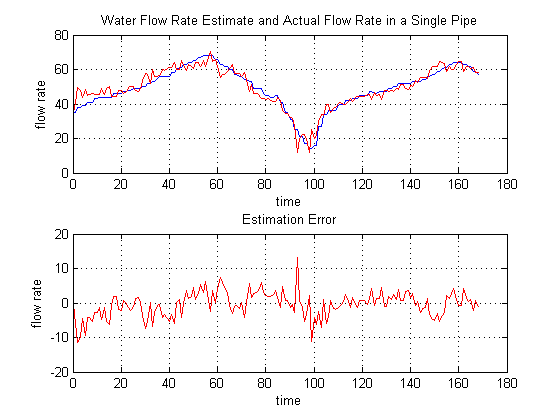
\includegraphics[width=80mm]{.//figures/singlepipe.png}
\caption{Water Flow Rate Estimate in a single pipe}
\vskip -6pt
\end{figure}

This subsection elaborates step-by-step validation of the models shown in section ??. First, section 5.2.1 validates equation () by comparing several models. To show its performance, we also give the evaluation against the ground truth. Section 5.2.2 shows propagation model validation through some experimental result. Section 5.2.3 shows its data after solving the optimization problem and shows how it looks like.

\begin{figure}
\centering
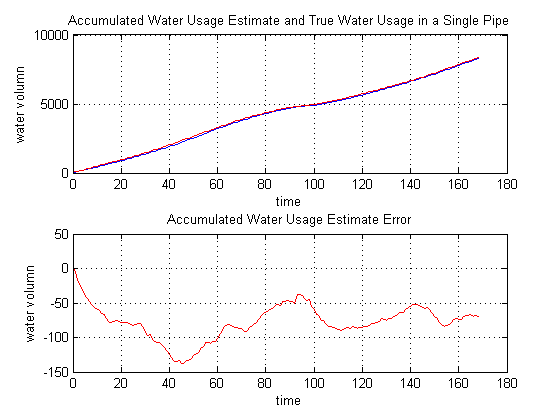
\includegraphics[width=80mm]{.//figures/singlepipe2.png}
\caption{Accumulated water usage in a single pipe}
\vskip -6pt
\end{figure}

\subsubsection{ Vibration to Water Flow Rate Model Validation }
From the equation (), one may expect the vibration to the water flow rate relation is linear. However, unmodelled parameters and sensor characteristics make the relationship nonlinear as shown in the figure. Getting a realistic model that well fits to the real relation is of importance to minimize the estimation error. Many model can be derived from the observation but decision relies on our heuristics. Most popular model for the curve fitting is polynomial curve fitting, but figure ?? shows saturation which is similar to square root curve or log curve. For comparison, we picked a 4th order polynomial fitting and 3rd root fitting shown in equation ??. We discarded log model to make the optimization problem solvable. 

\subsubsection{ Vibration Propagation among pipes }
As mentioned in section, we also validated that vibration propagation happens among pipes and can be approximated with the model given in equation (). 
To see the propagation from pipe 1 to pipe 2 and 3, we only turned on each of pipes at a time and plotted vibration on pipe i versus vibration on pipe j. Figures ??,??,?? and ?? show that the propagation can be approximated with a multiplicative coefficient. It comes with big variation that results in the water flow rate estimate error. (how do you).

\subsubsection{ Data Representation }

\begin{figure}
\centering
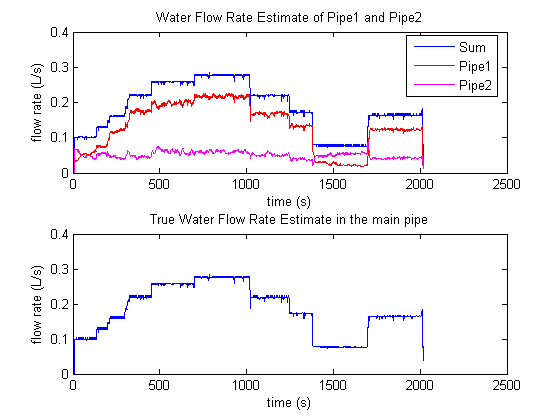
\includegraphics[width=80mm]{.//figures/twopipe.png}
\caption{Water Flow Rate Estimate of pipe 1 and 2}
\vskip -6pt
\end{figure}

Figures ?? and ?? give an example of water flow rate estimate of two pipes. Two metrics are considered because instant water flow rate estimate and accumulated water usage are both important. In figure ??, lower plot shows the water flow rate in the main pipe from the water flow meter. In the upper plot, blue line shows the sum of both pipies� water flow rate estimate, red line shows water flow rate estimate of pipe 1, and magenta line shows water flow rate estimate of pipe 2. Since we aim to minimize the sum of water flow rate estimate error, we can see in the figure that the sum of water flow rate estimate and the true water flow rate is the same as the system normalized the estimate based on the main water flow meter.
Similarly, figure ?? shows the accumulated water usage estimate from the figure. And two blue lines in the upper and lower figures are the same because of equation()


\begin{figure}
\centering
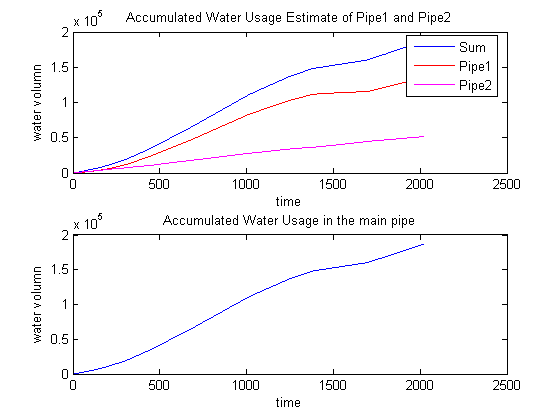
\includegraphics[width=80mm]{.//figures/twopipe2.png}
\caption{Accumulated water usage estimate of pipe 1 and 2}
\vskip -6pt
\end{figure}
